% !TEX TS-program = pdflatex
% !TEX encoding = UTF-8 Unicode

% This is a simple template for a LaTeX document using the "article" class.
% See "book", "report", "letter" for other types of document.

\documentclass[11pt]{article} % use larger type; default would be 10pt

\usepackage[utf8]{inputenc} % set input encoding (not needed with XeLaTeX)

%%% Examples of Article customizations
% These packages are optional, depending whether you want the features they provide.
% See the LaTeX Companion or other references for full information.

%%% PAGE DIMENSIONS
\usepackage{geometry} % to change the page dimensions
\geometry{a4paper} % or letterpaper (US) or a5paper or....
\geometry{margin=1in} % for example, change the margins to 2 inches all round
% \geometry{landscape} % set up the page for landscape
%   read geometry.pdf for detailed page layout information

\usepackage{graphicx} % support the \includegraphics command and options

% \usepackage[parfill]{parskip} % Activate to begin paragraphs with an empty line rather than an indent
\usepackage{amssymb}
\usepackage{amsmath}
%%% PACKAGES
\usepackage{booktabs} % for much better looking tables
\usepackage{array} % for better arrays (eg matrices) in maths
\usepackage{paralist} % very flexible & customisable lists (eg. enumerate/itemize, etc.)
\usepackage{verbatim} % adds environment for commenting out blocks of text & for better verbatim
\usepackage{subfig} % make it possible to include more than one captioned figure/table in a single float
% These packages are all incorporated in the memoir class to one degree or another...

%%% HEADERS & FOOTERS
\usepackage{fancyhdr} % This should be set AFTER setting up the page geometry
\pagestyle{fancy} % options: empty , plain , fancy
\renewcommand{\headrulewidth}{0pt} % customise the layout...
\lhead{}\chead{}\rhead{}
\lfoot{}\cfoot{\thepage}\rfoot{}

%%% SECTION TITLE APPEARANCE
\usepackage{sectsty}
\allsectionsfont{\sffamily\mdseries\upshape} % (See the fntguide.pdf for font help)
% (This matches ConTeXt defaults)

%%% ToC (table of contents) APPEARANCE
\usepackage[nottoc,notlof,notlot]{tocbibind} % Put the bibliography in the ToC
\usepackage[titles,subfigure]{tocloft} % Alter the style of the Table of Contents
\usepackage{bbm}
\usepackage{endnotes}

\renewcommand{\cftsecfont}{\rmfamily\mdseries\upshape}
\renewcommand{\cftsecpagefont}{\rmfamily\mdseries\upshape} % No bold!
\DeclareMathOperator*{\argmax}{arg\,max}
\DeclareMathOperator*{\argmin}{arg\,min}
\usepackage{graphicx}
\graphicspath{ {./pings/} }

\newcount\colveccount
\newcommand*\colvec[1]{
        \global\colveccount#1
        \begin{pmatrix}
        \colvecnext
}
\def\colvecnext#1{
        #1
        \global\advance\colveccount-1
        \ifnum\colveccount>0
                \\
                \expandafter\colvecnext
        \else
                \end{pmatrix}
        \fi
}

\newcommand{\norm}[1]{\left\lVert#1\right\rVert}

\title{Econometrics HW6}
\author{Michael B. Nattinger\footnote{I worked on this assignment with my study group: Alex von Hafften, Andrew Smith, and Ryan Mather. I have also discussed problem(s) with Emily Case, Sarah Bass, Katherine Kwok, and Danny Edgel.}}

\begin{document}
\maketitle

\section{Question 1}
\subsection{Part i}
$\hat{\mu}_{ols}$ can be computed as the average of all observations in the sample:
\begin{align*}
\hat{\mu}_{ols} &= \frac{1}{\sum_{i=1}^n T_i }\sum_{i=1}^n\sum_{t=1}^{T_i} Y_{it}\\
&= \frac{\sum_{i=1}^{n}1_{i}'Y_i}{\sum_{i=1}^{n}1_i'1_i}.
\end{align*}
\subsection{Part ii}
We write the estimator as signal plus noise:
\begin{align*}
\hat{\mu}_{iv} &= \frac{\sum_{i=1}^n Z_i'Y_i}{\sum_{i=1}^n Z_i'1_i}\\
&= \frac{\sum_{i=1}^n Z_i'(\mu_01_{i} + \alpha_i1_i + \epsilon_{i})}{\sum_{i=1}^n Z_i'1_i}\\
&= \mu_0 + \frac{\sum_{i=1}^n Z_i'(\alpha_i 1_i+ \epsilon_{i})}{\sum_{i=1}^n Z_i'1_i}.
\end{align*}

Now, we can find the variance:
\begin{align*}
Var(\hat{\mu}_{iv}) &= Var\left( \frac{\sum_{i=1}^n Z_i'(\alpha_i1_i + \epsilon_{i})}{\sum_{i=1}^n Z_i'1_i}\right)\\
&=   \frac{\sum_{i=1}^n Z_i'Var(\alpha_i1_i + \epsilon_{i})Z_i}{(\sum_{i=1}^n Z_i'1_i)^2}\\
&= \frac{\sum_{i=1}^n Z_i'\Omega_iZ_i}{(\sum_{i=1}^n Z_i'1_i)^2},
\end{align*}
where 
\begin{align*}
\Omega_i &= Var(\alpha_i1_i + \epsilon_{i})\\
&= \sigma_{\alpha}^21_i1_i' + \sigma^2I_{T_i}\\
&= \sigma_{\alpha}^21_i1_i' + \sigma^2I_{T_i}.
\end{align*}

\subsection{Part iii}
We will apply Cauchy-Schwarz. 
\begin{align*}
Z_{i}'1_i = Z_i'\Omega_i^{1/2}\Omega_i^{-1/2}\leq ||Z_i\Omega_i^{1/2}|| ||\Omega_i^{-1/2}1_i ||,\\
\left( \sum_{i=1}^n Z_i'1_i \right)^2 \leq \left( \sum_{i=1}^n ||\Omega_i^{1/2}Z_i||||\Omega_i^{-1/2}1_i|| \right)^2 \leq \sum_{i=1}^n Z_i'\Omega_i Z_i \cdot \sum_{i=1}^n 1_i'\Omega_i^{-1}1_i.
\end{align*}
We then apply the latter to the formula for variance and get:
\begin{align*}
Var(\hat{\mu}_{iv}) \geq \frac{\sum_{i=1}^nZ_i'\Omega_iZ_i}{\sum_{i=1}^nZ_i'\Omega_iZ_i \sum_{i=1}^nZ_i'\Omega_i^{-1}Z_i}
\end{align*}

If we use $\tilde{Z}_i = \Omega_i^{-1}1_i$ as an instrument then that has variance:
\begin{align*}
\frac{\sum_{i=1}^{n}\tilde{Z}_i\Omega_i\tilde{Z}_i}{(\sum_{i=1}^n \tilde{Z}_i'1_i)^2} &= \frac{1}{\sum_{i=1}^n 1_i'\Omega_i'1_i}
\end{align*}
\subsection{Part iv}
GLS and OLS are the same estimators when the panel is balanced. Therefore, GLS is not more efficient.

\begin{align*}
\Omega_i^{-1} &= \frac{1}{\sigma^2}I_{T_i} - \frac{1}{\sigma4}\frac{\sigma^2_aI_{T_i}1_i1_i'I_{T_i}}{1+\sigma_a^21'_iI_{T_i}1_i/\sigma^2} = \frac{1}{\sigma^2}\left( I_{T_i} - \frac{T_i\sigma^2_{a}}{T_i\sigma^2_a + \sigma^2}\frac{1_i1_i'}{T_i} \right)
\end{align*}

\begin{align*}
\tilde{Z}_i = \Omega_i^{-1}1_i = \frac{1_i}{T_i\sigma_a^2 + \sigma^2}.
\end{align*}
Now we impose $T_i = T$:
\begin{align*}
\hat{\mu}_{gls} = \frac{\sum \tilde{Z}_i'Y_i}{\tilde{Z}_i'1_i} = \frac{\sum \frac{1}{T\sigma_a^2 + \sigma^2}1_i'Y_i}{\sum \frac{1}{T\sigma_a^2 + \sigma^2}1_i'1_i} =  \frac{\sum 1_i'Y_i}{\sum1_i'1_i} = \hat{\mu}_{ols}.
\end{align*}
\subsection{Part v}
Let $\bar{\epsilon}_i = \frac{1}{T_i}\sum_{t=1}^{T_i}\epsilon_{it}$.
\begin{align*}
\hat{\sigma}^2_i &= \frac{1}{T_i - 1}\sum_{t=1}^{T_i}(Y_{it} -\bar{Y}_i)^2\\
&= \frac{1}{T_i - 1}\sum_{t=1}^{T_i}(\epsilon_{it} -\bar{\epsilon}_i)^2 \\
&= \frac{1}{T_i - 1}\sum_{t=1}^{T_i}\epsilon_{it}(\epsilon_{it} -\bar{\epsilon}_i)\\
&= \frac{1}{T_i - 1}\sum_{t=1}^{T_i}\epsilon_{it}^2 - \frac{1}{T_i(T_i - 1)}\sum_{t=1}^{T_i}\sum_{s=1}^{T_i}\epsilon_{is}\epsilon_{it}\\
&= \frac{1}{T_i }\sum_{t=1}^{T_i}\epsilon_{it}^2 - \frac{1}{T_i(T_i - 1)}\sum_{t=1}^{T_i}\sum_{s=1,s\neq t}^{T_i}\epsilon_{is}\epsilon_{it}.
\end{align*}

Therefore,
\begin{align*}
E[\hat{\sigma}^2_i] &= \frac{1}{T_i }\sum_{t=1}^{T_i}E[\epsilon_{it}^2]\\
&= \sigma^2.
\end{align*}

The estimator $\hat{\sigma}^2$ is an average of independent random variables, so under very mild assumptions (existence of fourth moment), consistency holds.
\subsection{Part vi}

\begin{align*}
E[\hat{\sigma}^2_{\alpha,i}(\mu)] &= E\left[\frac{1}{T_i}\sum_{t=1}^{T_i}(Y_{it} -\mu)^2 - \hat{\sigma}_i^2\right]\\
&=  E\left[\frac{1}{T_i}\sum_{t=1}^{T_i}(\alpha_{i} + \epsilon_{it})^2 - \hat{\sigma}_i^2\right]\\
&= E\left[\frac{1}{T_i}\sum_{t=1}^{T_i}(\alpha_{i}^2 +2 \alpha_i\epsilon_{it} + \epsilon_{it}^2)\right] - \sigma^2\\
&= \sigma^2_{\alpha} + \sigma^2 - \sigma^2\\
&= \sigma^2_{\alpha}
\end{align*}

By the same logic as in part (v), we have the average of uncorrelated random variables as our estimator, so the estimator is consistent under very mild assumptions.
\subsection{Part vii}

Extending (iv),
\begin{align*}
\left( \sum_{i=1}^n 1_i'\Omega_i^{-1}1_i\right)^{-1} = \left( \sum_{i=1}^n \frac{T_i}{T_i\sigma_{\alpha}^2 + \sigma^2} \right)^{-1}
\end{align*}
We can use a plug-in estimator,
\begin{align*}
\hat{V} &= \left( \sum_{i=1}^n \frac{T_i}{T_i\hat{\sigma}_{\alpha}^2 + \hat{\sigma}^2} \right)^{-1}.
\end{align*}

This will be consistent by the continuous mapping theorem.
\section{Question 2}
\subsection{Part i}
\begin{align*}
\hat{\beta}_{FE} &\rightarrow_p \beta_0 + \frac{E[\sum_{t=1}^T (X_{it} - \bar{X}_i)\epsilon_{it}]}{E[\sum_{t=1}^T(X_{it} - \bar{X}_i)^2]}\\
&=  \beta_0 + \frac{E[\sum_{t=1}^T X_{it}\epsilon_{it}] - E[\sum_{t=1}^T\bar{X}_i\epsilon_{it}]}{(T-1)\sigma_x^2} \\
&=  \beta_0 + \frac{- E[\sum_{t=1}^T\bar{X}_i\epsilon_{it}]}{(T-1)\sigma_x^2} \\
&= \beta_0 + \frac{- E[\sum_{t=1}^T\sum_{s=1}^TX_{is}\epsilon_{it}]}{T(T-1)\sigma_x^2}\\ 
&= \beta_0 + \frac{- (T-1)\delta\sigma^2_x}{T(T-1)\sigma_x^2}\\
&= \beta_0 - \frac{\delta}{T}
\end{align*}

Therefore, the asymptotic bias of $\hat{\beta}_{FE}$ is $-\frac{\delta}{T}$.

\begin{align*}
\hat{\beta}_{FD} &\rightarrow_p \beta_0 + \frac{E[\sum_{t=2}^T (X_{it} - X_{i,t-1})(\epsilon_{it} - \epsilon_{i,t-1})]}{E[\sum_{t=1}^T(X_{it} - X_{i,t-1})^2]}\\
&= \beta_0 + \frac{E[\sum_{t=2}^T X_{it}\epsilon_{it} - X_{i,t-1}\epsilon_{it} -X_{it}\epsilon_{i,t-1} + X_{i,t-1}\epsilon_{i,t-1} ]}{E[\sum_{t=2}^TX^2_{it} - 2X_{it}X_{i,t-1} + X_{i,t-1}^2]}\\
&= \beta_0 + \frac{-(T-1)\delta \sigma_{x}^2  }{2(T-1)\sigma_x^2}\\
&= \beta_0 + \frac{-\delta  }{2}
\end{align*}

Therefore, the asymptotic bias of $\hat{\beta}_{FD}$ is $-\frac{\delta}{2}$.

\subsection{Part ii}

For $T=2$, the asymptotic biases are the same.
\section{Question 3}
\subsection{Part i}
We run the simulation a single time, output is below:

\begin{center}
\begin{tabular}{llllllllll}
& FE & OLS & $\delta_2$ & $\delta_3$ & $\delta_4$ & EW LB & EW UB & C LB & C UB \\ 
\hline 
$\phi=0,n=40$ & 1.28 & 2.79 & 1.1 & 0.815 & 0.943 & 0.685 & 1.87 & 0.56 & 2 \\ 
$\phi=0.8,n=40$ & 0.775 & 2.4 & 1.22 & 1.14 & 1.2 & 0.227 & 1.32 & -0.103 & 1.65 \\ 
$\phi=0,n=70$ & 0.527 & 2.25 & 1.02 & 1.31 & 1.19 & 0.0732 & 0.982 & 0.0256 & 1.03 \\ 
$\phi=0.8,n=70$ & 0.441 & 2.24 & 1.01 & 1.08 & 1.04 & 0.0546 & 0.828 & -0.15 & 1.03 \\ 
$\phi=0,n=100$ & 0.846 & 2.69 & 1.13 & 1.22 & 1.13 & 0.508 & 1.18 & 0.489 & 1.2 \\ 
$\phi=0.8,n=100$ & 1.15 & 2.94 & 1.01 & 0.939 & 0.879 & 0.836 & 1.47 & 0.663 & 1.64 \\ 
\hline 
\end{tabular}
\end{center}

\subsection{Part ii}
We run the simulation 10000 times. The output is below, and code follows at the end of the problem set:
\begin{center}
\begin{tabular}{lllll}
& FE & OLS & EW & Cluster \\ 
\hline 
$\phi=0,n=40$ & 0.999 & 2.67 & 0.894 & 0.92 \\ 
$\phi=0.8,n=40$ & 1.01 & 2.68 & 0.79 & 0.919 \\ 
$\phi=0,n=70$ & 1 & 2.67 & 0.902 & 0.938 \\ 
$\phi=0.8,n=70$ & 1 & 2.67 & 0.807 & 0.935 \\ 
$\phi=0,n=100$ & 1 & 2.68 & 0.9 & 0.939 \\ 
$\phi=0.8,n=100$ & 0.996 & 2.67 & 0.811 & 0.938 \\ 
\hline 
\end{tabular}
\end{center}

\subsection{Part iii}
Our Monte-Carlo results demonstrate that the fixed effects estimation is unbiased, whereas the (incorrectly specified) OLS estimated coefficient is badly upwardly biased. It also demonstrates that the cluster standard errors have a coverage rate much closer to the correct value than the heteroskedasticity robust standard errors.  The cluster standard errors are just as robust in the case without autocorrelation in the error term as they are with autocorrelation, whereas the heteroskedasticity robust standard errors lose a lot of coverage in that case.

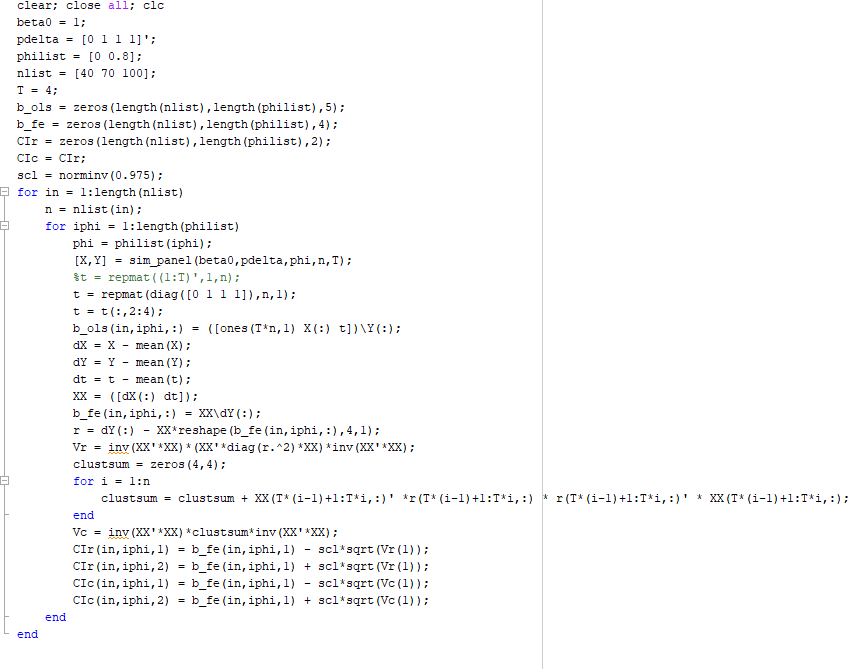
\includegraphics{hw6p1}

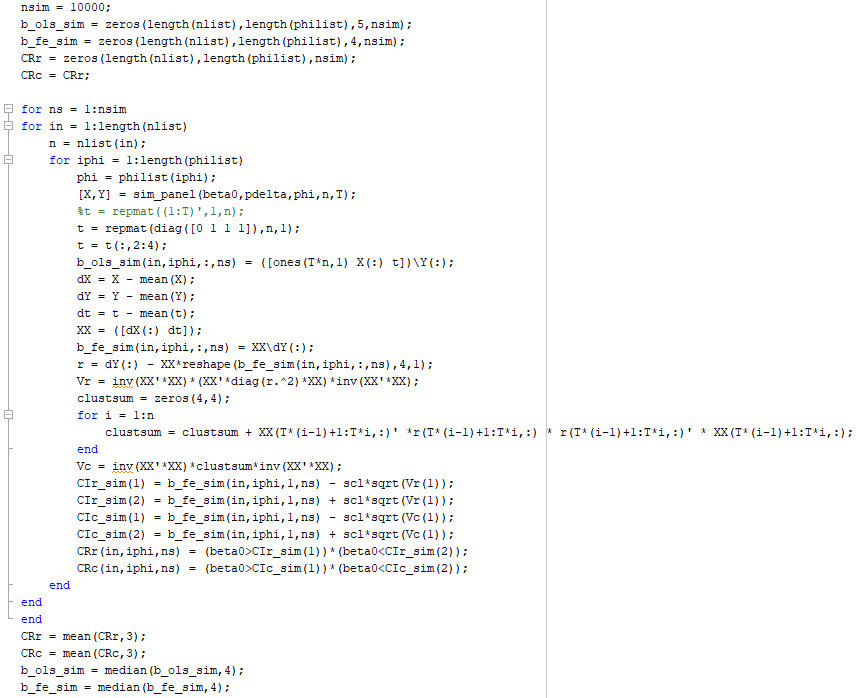
\includegraphics{hw6p2}

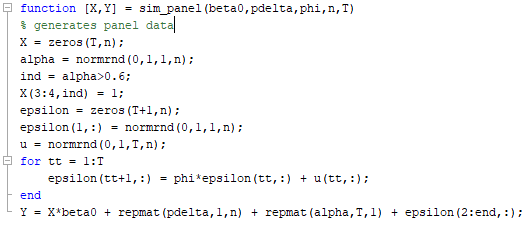
\includegraphics{hw6p3}
\end{document}
